\documentclass[12pt]{article}
\usepackage{graphicx}
\graphicspath{ {./images/} }
\usepackage[utf8]{inputenc}
\usepackage{amsfonts,latexsym,amsthm,amssymb,amsmath,amscd,euscript}
\usepackage{ragged2e} %To align text.
\usepackage{fullpage} %Automatically set the margin
\usepackage{hyperref}
    \hypersetup{colorlinks=true,citecolor=blue,urlcolor =black,linkbordercolor={1 0 0}}
\author{Suryansh Shukla}
\date{\today}

%%%%%%%%%%Title%%%%%%%%%%
\title{Notes Template}
%%%%%%%%%%%%%%%%%%%%%%%%
\begin{document}
\maketitle
\tableofcontents
\newpage

%%%%%%%%%%Questions%%%%%%%%%%
\section{Questions}
\textbf{
\begin{enumerate}
    \item What is the first question?
    \item What is the second question?
\end{enumerate}
}
\newpage
%%%%%%%%%%%%%%%%%%%%%%%%

\section{Section 2}
\subsection{Subsection}

Table of content is very important for thinking. 
The first section can be of Questions. 
And after that we can start with the next page of notes. 

\section{Adding bibliography}
\cite{Wu}

\section{Adding Image}


\begin{figure}[h!]
    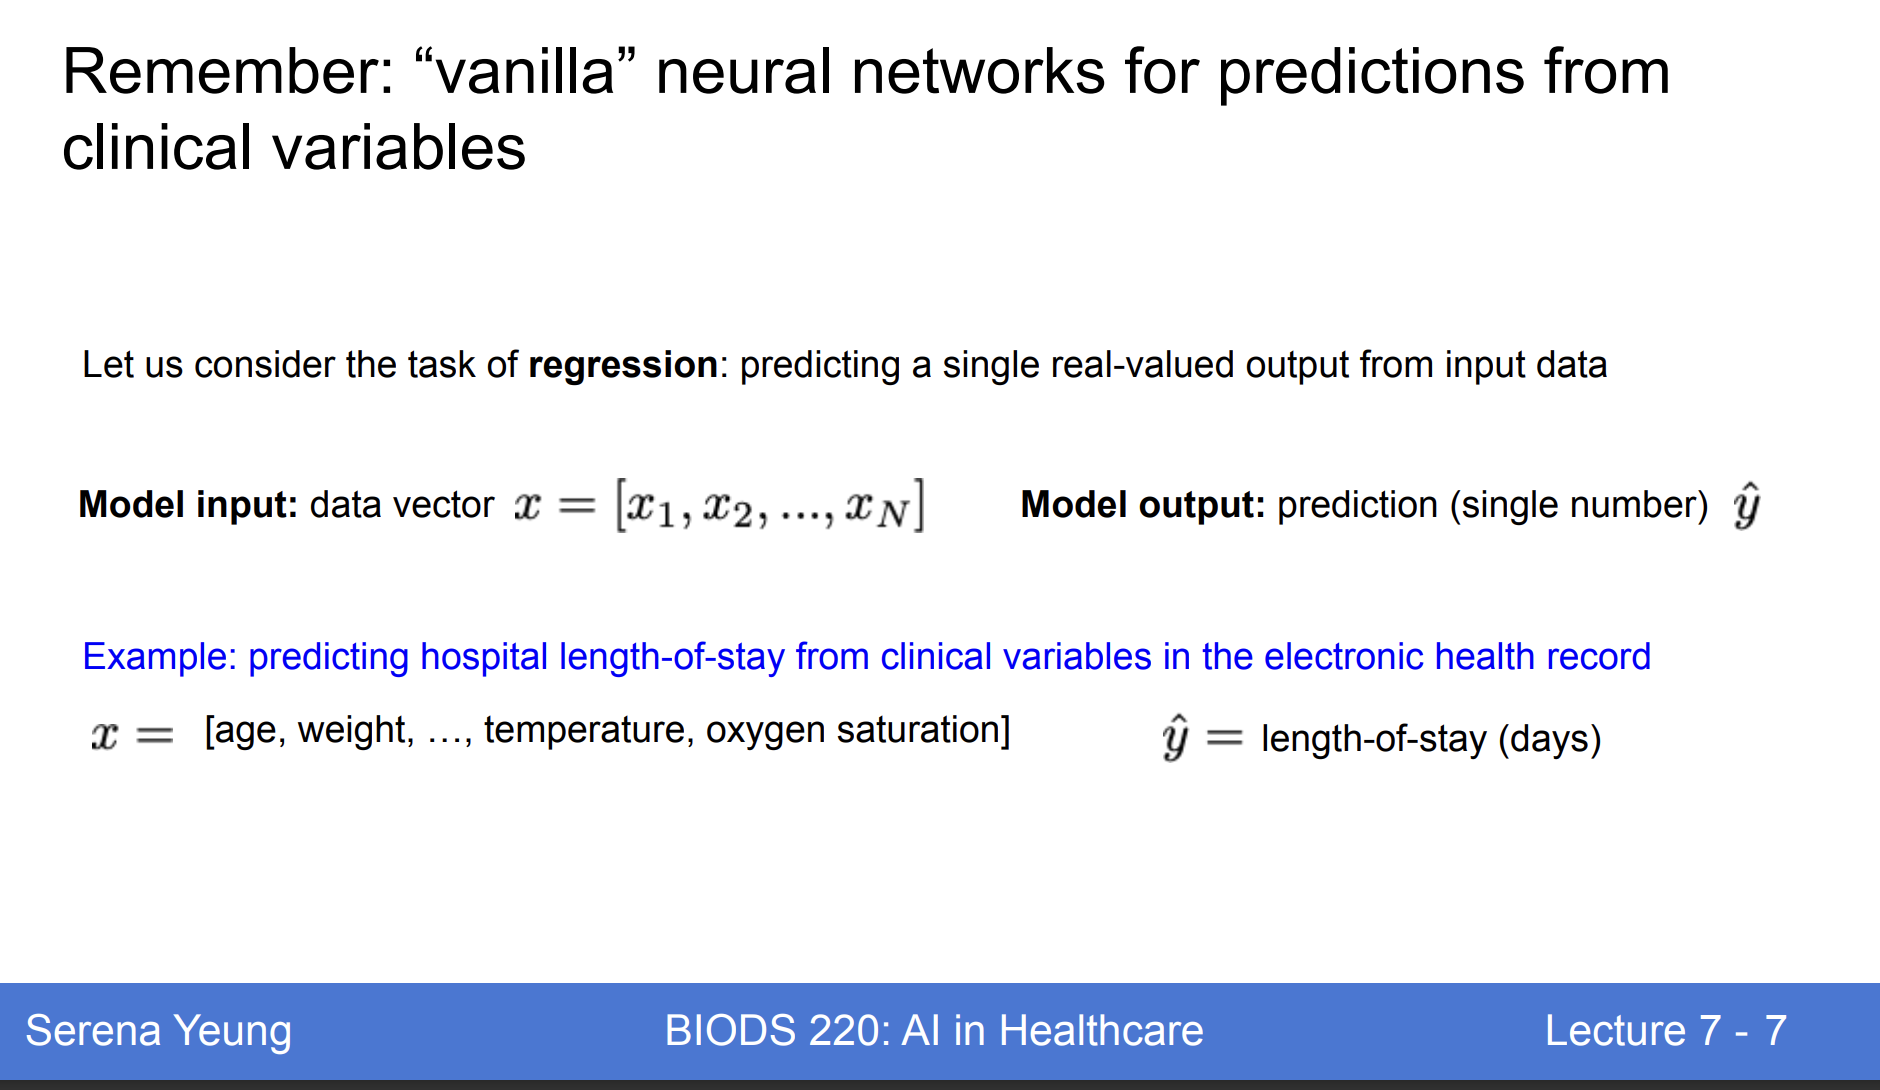
\includegraphics[scale=.5]{image1.png}
\end{figure}


%%%%%%%%%%Bibliography%%%%%%%%%%
\newpage
\bibliographystyle{plain}
\bibliography{bibliography.bib}
%%%%%%%%%%%%%%%%%%%%%%%%


\end{document}
